\section{Design esperimenti}



\noindent Il lavoro svolto consiste nel: 
\begin{itemize}
    \item valutare e prevedere l'impatto ambientale di un sistema di raccomandazione (RecSys) in base alla sua sostenibilità
    \item cercare una soluzione per ridurre l'impatto ambientale di un RecSys senza però perdere di performance in modo significativo.
\end{itemize}

\noindent Nella prima parte dunque sono stati effettuati ulteriori esperimenti per valutare l'impatto ambientale di diversi modelli di raccomandazione su diversi dataset. Questi dati sono stati utilizzati per addestrare un modello di regressione che permette di prevedere le emissioni prodotte da un modello di raccomandazione in base a diversi parametri.


\noindent Nella seconda parte, invece, ci si è concentrati su come ridurre l'impatto ambientale di un RecSys senza però perdere di performance. In particolare, si è cercato di capire se fosse possibile ridurre le emissioni prodotte da un modello di raccomandazione senza però perdere di performance in modo significativo.



\noindent Per quanto riguarda la valutazione, mediante la libreria CodeCarbon\footnote{\href{http://codecarbon.io}{CodeCarbon}}{} è stato possibile misurare le emissioni prodotte dalla macchina durante l'addestramento con parametri di default per un dato modello dato un dataset. 
In questo ambito  Spillo et al.\cite{spillo2023towards} mostrano come spesso algoritmi più semplici riescono ad avere delle performance molto simili a modelli più complessi, ma con un impatto ambientale decisamente minore.

\begin{figure}[H]
    \centering
    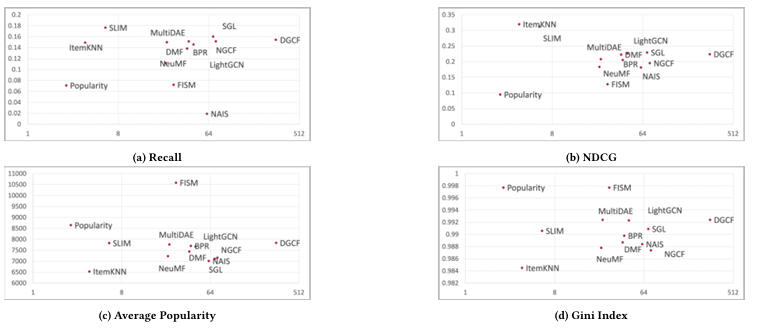
\includegraphics[scale=0.75]{images/risultati-valutazione.png}
    \caption{Trade-off tra emissioni e performance con dataset Mind}


\end{figure}
\newpage




